% 1p

\subsubsection{Cost Function}
% 0.5P
To build the cost function, we use the cross-entropy between the training data and the model’s predictions. The total cost function combine the primary cost function with a regularization term.

\subsubsubsection{Learning Conditional Distributions with Maximum Likelihood}
% 1.25p
Cost function is the negative log-likelihood, equivalently described as the cross-entropy between the training data and the model distribution.

  % eq 6.12
  \begin{equation} \tag{6.12}
   \label{eq_6_12}
    J( \bm{\theta} ) = - \mathbb{E} _ {\bm{\mathrm{x}}, \bm{\mathrm{y}} \sim \hat{p} _ \mathrm{data} } 
          \log p _ \mathrm{model} ( \bm{y}\ |\ \bm{x} )
  \end{equation}

The cost function changes depending on the specific form of $\log p _ \mathrm{model}$.
if $p _ \mathrm{model}(\bm{y}\ |\ \bm{x}) = \mathcal{N}(\bm{y}; f(\bm{x}; \bm{\theta}), \bm{I})$

  % eq 6.13
  \begin{equation} \tag{6.13}
   \label{eq_6_13}
    J( \theta ) = \frac{1}{2} \mathbb{E} _ {\bm{\mathrm{x}}, \bm{\mathrm{y}} \sim \hat{p}_ \mathrm{data}}
        \| \bm{y} - f( \bm{x} ; \bm{\theta} ) \| ^ 2 + \mathrm{const}
  \end{equation}

\subsubsubsection{Learning Conditional Statistics}
% 1.25p
Using calculus of variations to solve the optimization problem.
First result:

  % eq 6.14
  \begin{equation} \tag{6.14}
   \label{eq_6_14}
   f ^ * = {\arg \min} _ {f} \mathbb{E} _ {\bm{\mathrm{x}}, \bm{\mathrm{y}} \sim p _ \mathrm{data}} 
       \| \bm{y} - f( \bm{x} ) \| ^ 2
  \end{equation}
  
  % eq 6.15
  \begin{equation} \tag{6.15}
   \label{eq_6_15}
    f ^ * (\bm{x}) = \mathbb{E} _ {\bm{\mathrm{y}} \sim p _ \mathrm{data} ( \bm{y} | \bm{x} ) } [ \bm{y} ]
  \end{equation}
  
Second result:

  % eq 6.16
  \begin{equation} \tag{6.16}
   \label{eq_6_16}
   f ^ * = {\arg \min} _ {f} \mathbb{E} _ {\bm{\mathrm{x}}, \bm{\mathrm{y}} \sim p _ \mathrm{data}} 
       \| \bm{y} - f( \bm{x} ) \| _ 1
%   \mathit{f}^*=\arg\min_{\mathit{f}}\ \mathbb{E}_{x,y\sim\mathit{p}_{data}}\|\bm{y}\ -\ \mathit{f}(\bm{x})\|_1
  \end{equation}

\subsubsection{Output Units}
% 0.5p
$\bm{h} = f( \bm{x}; \bm{\theta})$ defines a set of hidden features which is provided by the feedforward network.

\subsubsubsection{Linear Units for Gaussian Output Distributions}
% 0.5p
Linear output units produces a vector $\hat{\bm{y}} = \bm{W} ^ \top \bm{h} + \bm{b}$
Using Linear output layers to produce the mean of a conditional Gaussian distribution:

  % eq 6.17
  \begin{equation} \tag{6.17}
   \label{eq_6_17}
   p(\bm{y}\ |\ \bm{x}) = \mathcal{N}(\bm{y}; \hat{\bm{y}}, \bm{I})
  \end{equation}

\subsubsubsection{Sigmoid Units for Bernoulli Output Distributions}
% 2.25p
The neural net needs to predict only $P(y=1\ |\ \bm{x})$ in a Bernoulli distribution.
We use a linear unit and threshold its value to get a valid probability.

  % eq 6.18
  \begin{equation} \tag{6.18}
   \label{eq_6_18}
   P(y = 1\ |\ \bm{x}) = \max \{ 0, \min \{ 1, \bm{w} ^ \top \bm{h} + b \} \}
  \end{equation}
  
A sigmoid output unit:

  % eq 6.19
  \begin{equation} \tag{6.19}
    \label{eq_6_19}
    \hat{y} = \sigma( \bm{w} ^ \top \bm{h} + b)
  \end{equation}
  
Normalize to see this yields a Bernoulli distribution controlled by a sigmoidal transformation of z:

  % eq 6.20 ~ 6.23
  \setcounter{equation}{20}
  \begin{align} \tag{6.20}
   \label{eq_6_20}
    \log \tilde{P}(y)& =yz\\
    \tilde{P}(y)& = \exp(yz)\\
    P(y)& =\frac{\exp(yz)}{\sum _ {y'=0} ^ {1} \exp(y'z) }\\
    P(y)& =\sigma( (2y-1)z )
  \end{align}
  
The loss function for maximum likelihood learning of a Bernoulli parametrized by a sigmoid:

  % eq 6.24 ~ 6.26
  \setcounter{equation}{24}
  \begin{align} \tag{6.24}
   \label{eq_6_24}
    J(\bm{\theta})& = - \log P(y\ |\ \bm{x})\\
    & = - \log \sigma( (2y-1)z )\\
    & = \zeta( (1-2y)z )
  \end{align}

  \subsubsubsection{Softmax Units for Multinoulli Output Distributions}
  % 3.25p
  Softmax functions are often used as a classifier, to classified $n$ different classes.

  We want to generalize the Bernoulli distribution to multinoulli distribution.

  % eq 6.27
  \begin{equation} \tag{6.27}
    \label{eq_6_27}
    \hat{y} = P( y=1\ |\ \bm{x} )
  \end{equation}

  The~\eqref{eq_6_27} shows a example of maximum likelihood defined by Bernoulli distribution.
  Next, using log-likelihood to simplify computation. We take $z _ i = \log \tilde{P}( y=1\ |\ \bm{x} )$, so:

  % eq 6.28
  \begin{equation} \tag{6.28}
    \label{eq_6_28}
    \bm{z} = \bm{W} ^ \top \bm{h} + \bm{b}
  \end{equation}

  and apply softmax function:

  % eq 6.29
  \begin{equation} \tag{6.29}
    \label{eq_6_29}
    \mathrm{softmax}{( \bm{z} )} _ i = \frac{\ \exp(z_i) } {\ \sum _ j \exp(z_j) }
  \end{equation}
  % eq 6.30
  \begin{equation} \tag{6.30}
    \label{eq_6_30}
    \log\ \mathrm{softmax}{( \bm{z} )} _ i = z_i - \log \sum _ j \exp(z_j)
  \end{equation}

  Overall, we can approximate the model as:

  % eq 6.31
  \begin{equation} \tag{6.31}
    \label{eq_6_31}
    \mathrm{softmax}{( \bm{z}( \bm{x};\bm{\theta} ) )} _ i \approx
      \frac{\ \sum ^ m _ {j=1} \bm{1} _ {y ^ {(j)} = i, \bm{x} ^ {(j)} = \bm{x}} }
        {\ \sum ^ m _ {j=1} \bm{1} _ {\ \bm{x} ^ {(j)} = \bm{x}} }
  \end{equation}

  Like the sigmoid, the softmax function can saturate if the difference between its inputs is large.

  The softmax function's property:

  % eq 6.32
  \begin{equation} \tag{6.32}
    \label{eq_6_32}
    \mathrm{softmax}( \bm{z} ) = \mathrm{softmax}( \bm{z} + c )
  \end{equation}
  % eq 6.33
  \begin{equation} \tag{6.33}
    \label{eq_6_33}
    \mathrm{softmax}( \bm{z} ) = \mathrm{softmax}( \bm{z} - \max _ i (z _ i) )
  \end{equation}

  With~\eqref{eq_6_32} and~\eqref{eq_6_33}, we can evaluate small difference between each $z _ i$, even if $z _ i$ are large negative number.

  From neuroscience, the softmax becomes a form of \textbf{winner-take-all}.

\subsubsubsection{Other Output Types}
% 3.75p

  Cost function for generalized neural network:
  $p( \bm{y} \ |\ \bm{x};\bm{\theta} )$

  \begin{itemize}

%    \item{Heteroscedastic Model}
%
%    A model to predict
%
%    % eq 6.34
%    \begin{equation} \tag{6.34}
%      \label{eq_6_34}
%      diag(\bm{\beta})
%    \end{equation}

    \item{Mixture Density Networks}

    The Gaussian mixture output is defined as below:

    % eq 6.35
    \begin{equation} \tag{6.35}
      \label{eq_6_35}
      p( \bm{y}\ |\ \bm{x} ) =
        \sum ^ n _ {i=1} p( c=i\ |\ \bm{x} )
        \mathcal{N}( \bm{y}; \bm{\mu} ^ {(i)} (\bm{x}), \bm{\Sigma} ^ {(i)} (\bm{x}) )
    \end{equation}

    The neural network must provide outputs:

    \begin{itemize}

      \item{Mixture components $p(c = i\ |\ \bm{x})$:}

        A multinoulli distribution of $n$ different categories with potential variable $c$.

      \item{Means $\bm{\mu} ^ {(i)} (\bm{x})$:}

        The mean of $i$-th Gaussian distribution.

      \item{Covariances $\bm{\Sigma} ^ {(i)} (\bm{x})$:}

        The covariance matrix of $i$-th Gaussian distribution.

    \end{itemize}

      Using \textbf{clip gradients} in gradient-based optimization on numerically unstable neural networks.

    \newpage

    % fig 6.4
    \setcounter{figure}{3}
    \begin{figure}[ht]
      \begin{center}
        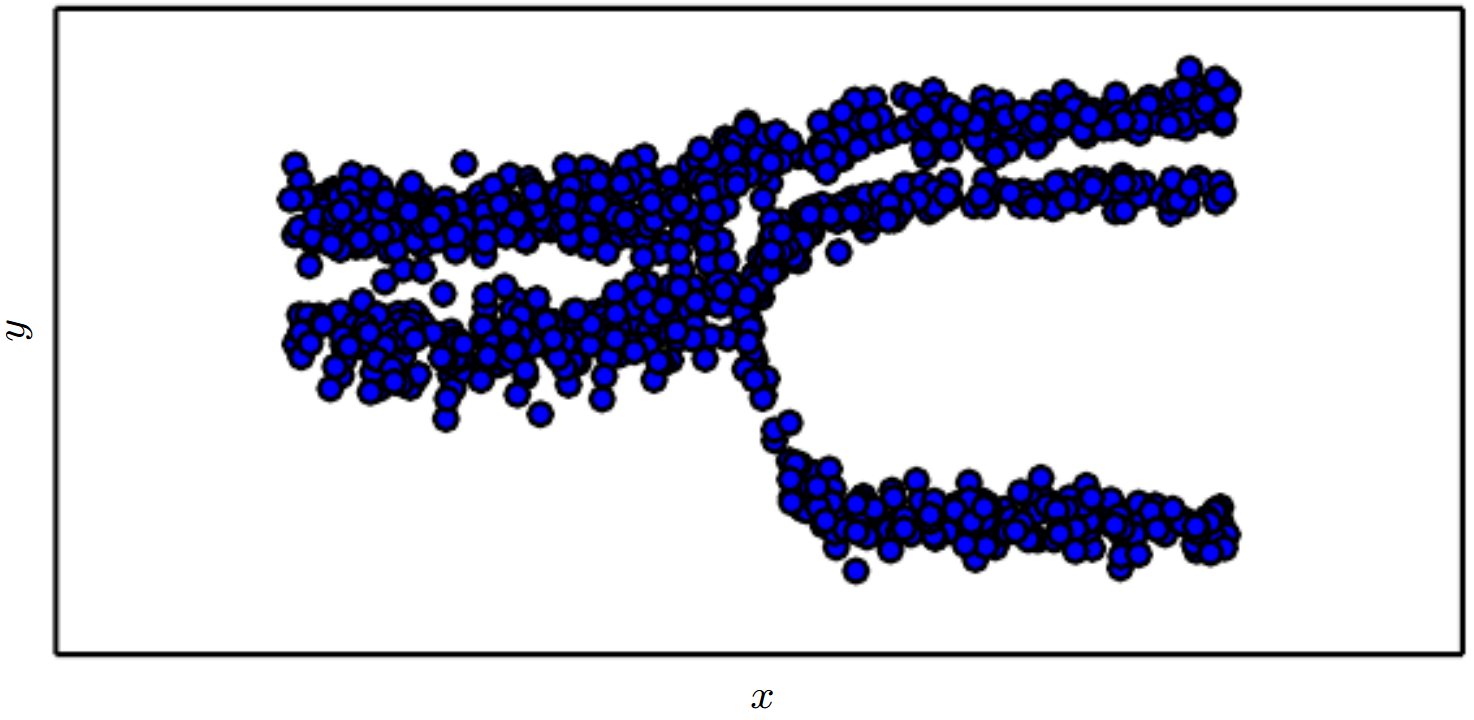
\includegraphics[width=0.8\textwidth]{FIG/fig6_4.PNG}
        \caption{Samples drawn from a neural network with a mixture density output layer.
          The input $x$ is sampled from a uniform distribution,
          and the output $y$ is sampled from $p _ {model} (y\ |\ x)$.
          The neural network is able to learn nonlinear mappings from the input to the parameters of the output distribution.
          These parameters include the probabilities governing which of three mixture components will generate the output as well as the parameters for each mixture component.
          Each mixture component is Gaussian with predicted mean and variance.
          All these aspects of the output distribution are able to vary with respect to the input $x$,
          and to do so in nonlinear ways.
        }\label{fig:NN_mixture_density_output_layer}
      \end{center}
    \end{figure}

    Figure~\ref{fig:NN_mixture_density_output_layer} is an example of mixture density network.

  \end{itemize}

